\documentclass[french,ignorenonframetext,]{beamer}
\usepackage{multimedia}
\usepackage{animate}
\setbeamertemplate{caption}[numbered]
\setbeamertemplate{caption label separator}{: }
\setbeamercolor{caption name}{fg=normal text.fg}
\beamertemplatenavigationsymbolsempty
\usepackage{lmodern}
\usepackage{amssymb,amsmath}
\usepackage{ifxetex,ifluatex}
\usepackage{fixltx2e} % provides \textsubscript
\ifnum 0\ifxetex 1\fi\ifluatex 1\fi=0 % if pdftex
  \usepackage[T1]{fontenc}
  \usepackage[utf8]{inputenc}
\else % if luatex or xelatex
  \ifxetex
    \usepackage{mathspec}
  \else
    \usepackage{fontspec}
    \usepackage{luatexja-fontspec}
  \fi
  \defaultfontfeatures{Ligatures=TeX,Scale=MatchLowercase}
    \setmainfont[]{Source Serif Pro}
    \setsansfont[]{Source Sans Pro}
    \setmonofont[Mapping=tex-ansi]{Source Code Pro}
\fi
\usefonttheme{serif} % use mainfont rather than sansfont for slide text
% use upquote if available, for straight quotes in verbatim environments
\IfFileExists{upquote.sty}{\usepackage{upquote}}{}
% use microtype if available
\IfFileExists{microtype.sty}{%
\usepackage{microtype}
\UseMicrotypeSet[protrusion]{basicmath} % disable protrusion for tt fonts
}{}
\ifnum 0\ifxetex 1\fi\ifluatex 1\fi=0 % if pdftex
  \usepackage[shorthands=off,main=french]{babel}
\else
  \usepackage{polyglossia}
  \setmainlanguage[]{french}
\fi
\newif\ifbibliography
\hypersetup{
            pdftitle={Génération de mouvement en robotique mobile et humanoïde},
            pdfauthor={Guilhem Saurel},
            pdfborder={0 0 0},
            breaklinks=true,unicode=true}
\urlstyle{same}  % don't use monospace font for urls
\usepackage{graphicx,grffile}
\makeatletter
\def\maxwidth{\ifdim\Gin@nat@width>\linewidth\linewidth\else\Gin@nat@width\fi}
\def\maxheight{\ifdim\Gin@nat@height>\textheight0.8\textheight\else\Gin@nat@height\fi}
\makeatother
% Scale images if necessary, so that they will not overflow the page
% margins by default, and it is still possible to overwrite the defaults
% using explicit options in \includegraphics[width, height, ...]{}
\setkeys{Gin}{width=\maxwidth,height=\maxheight,keepaspectratio}

% Prevent slide breaks in the middle of a paragraph:
\widowpenalties 1 10000
\raggedbottom

\AtBeginPart{
  \let\insertpartnumber\relax
  \let\partname\relax
  \frame{\partpage}
}
\AtBeginSection{
  \ifbibliography
  \else
    \let\insertsectionnumber\relax
    \let\sectionname\relax
    \frame{\sectionpage}
  \fi
}
\AtBeginSubsection{
  \let\insertsubsectionnumber\relax
  \let\subsectionname\relax
  \begin{frame}
  \tableofcontents[currentsubsection, hideothersubsections,
                   sectionstyle=show/shaded, subsectionstyle=show/shaded]
  \end{frame}
}

\setlength{\parindent}{0pt}
\setlength{\parskip}{6pt plus 2pt minus 1pt}
\setlength{\emergencystretch}{3em}  % prevent overfull lines
\providecommand{\tightlist}{%
  \setlength{\itemsep}{0pt}\setlength{\parskip}{0pt}}
\setcounter{secnumdepth}{5}

\title[]{Génération de mouvement en robotique mobile et humanoïde}
\author{Guilhem Saurel}
\institute{Gepetto - LAAS-CNRS}
\date{3 octobre 2017}

\begin{document}
\frame{\titlepage}

\begin{frame}
\tableofcontents
\end{frame}

\section{Introduction}\label{introduction}

\subsection{A Introduction}\label{a-introduction}

\begin{frame}{Robots mobiles et bipèdes}

La robotique consiste à créer des machines universelles, dans le sens où
elles peuvent éxécuter une large variété de tâches, y compris certaines
qui n'étaient pas prévues au moment de la conception.

Pour cela, un robot a besoin d'être capable de générer des mouvements de
manipulation et de locomotion. Dans cette thèse, nous avons étudié deux
modes de locomotion terrestre: le roulement sans glissements et la
marche.

\begin{figure}
\centering
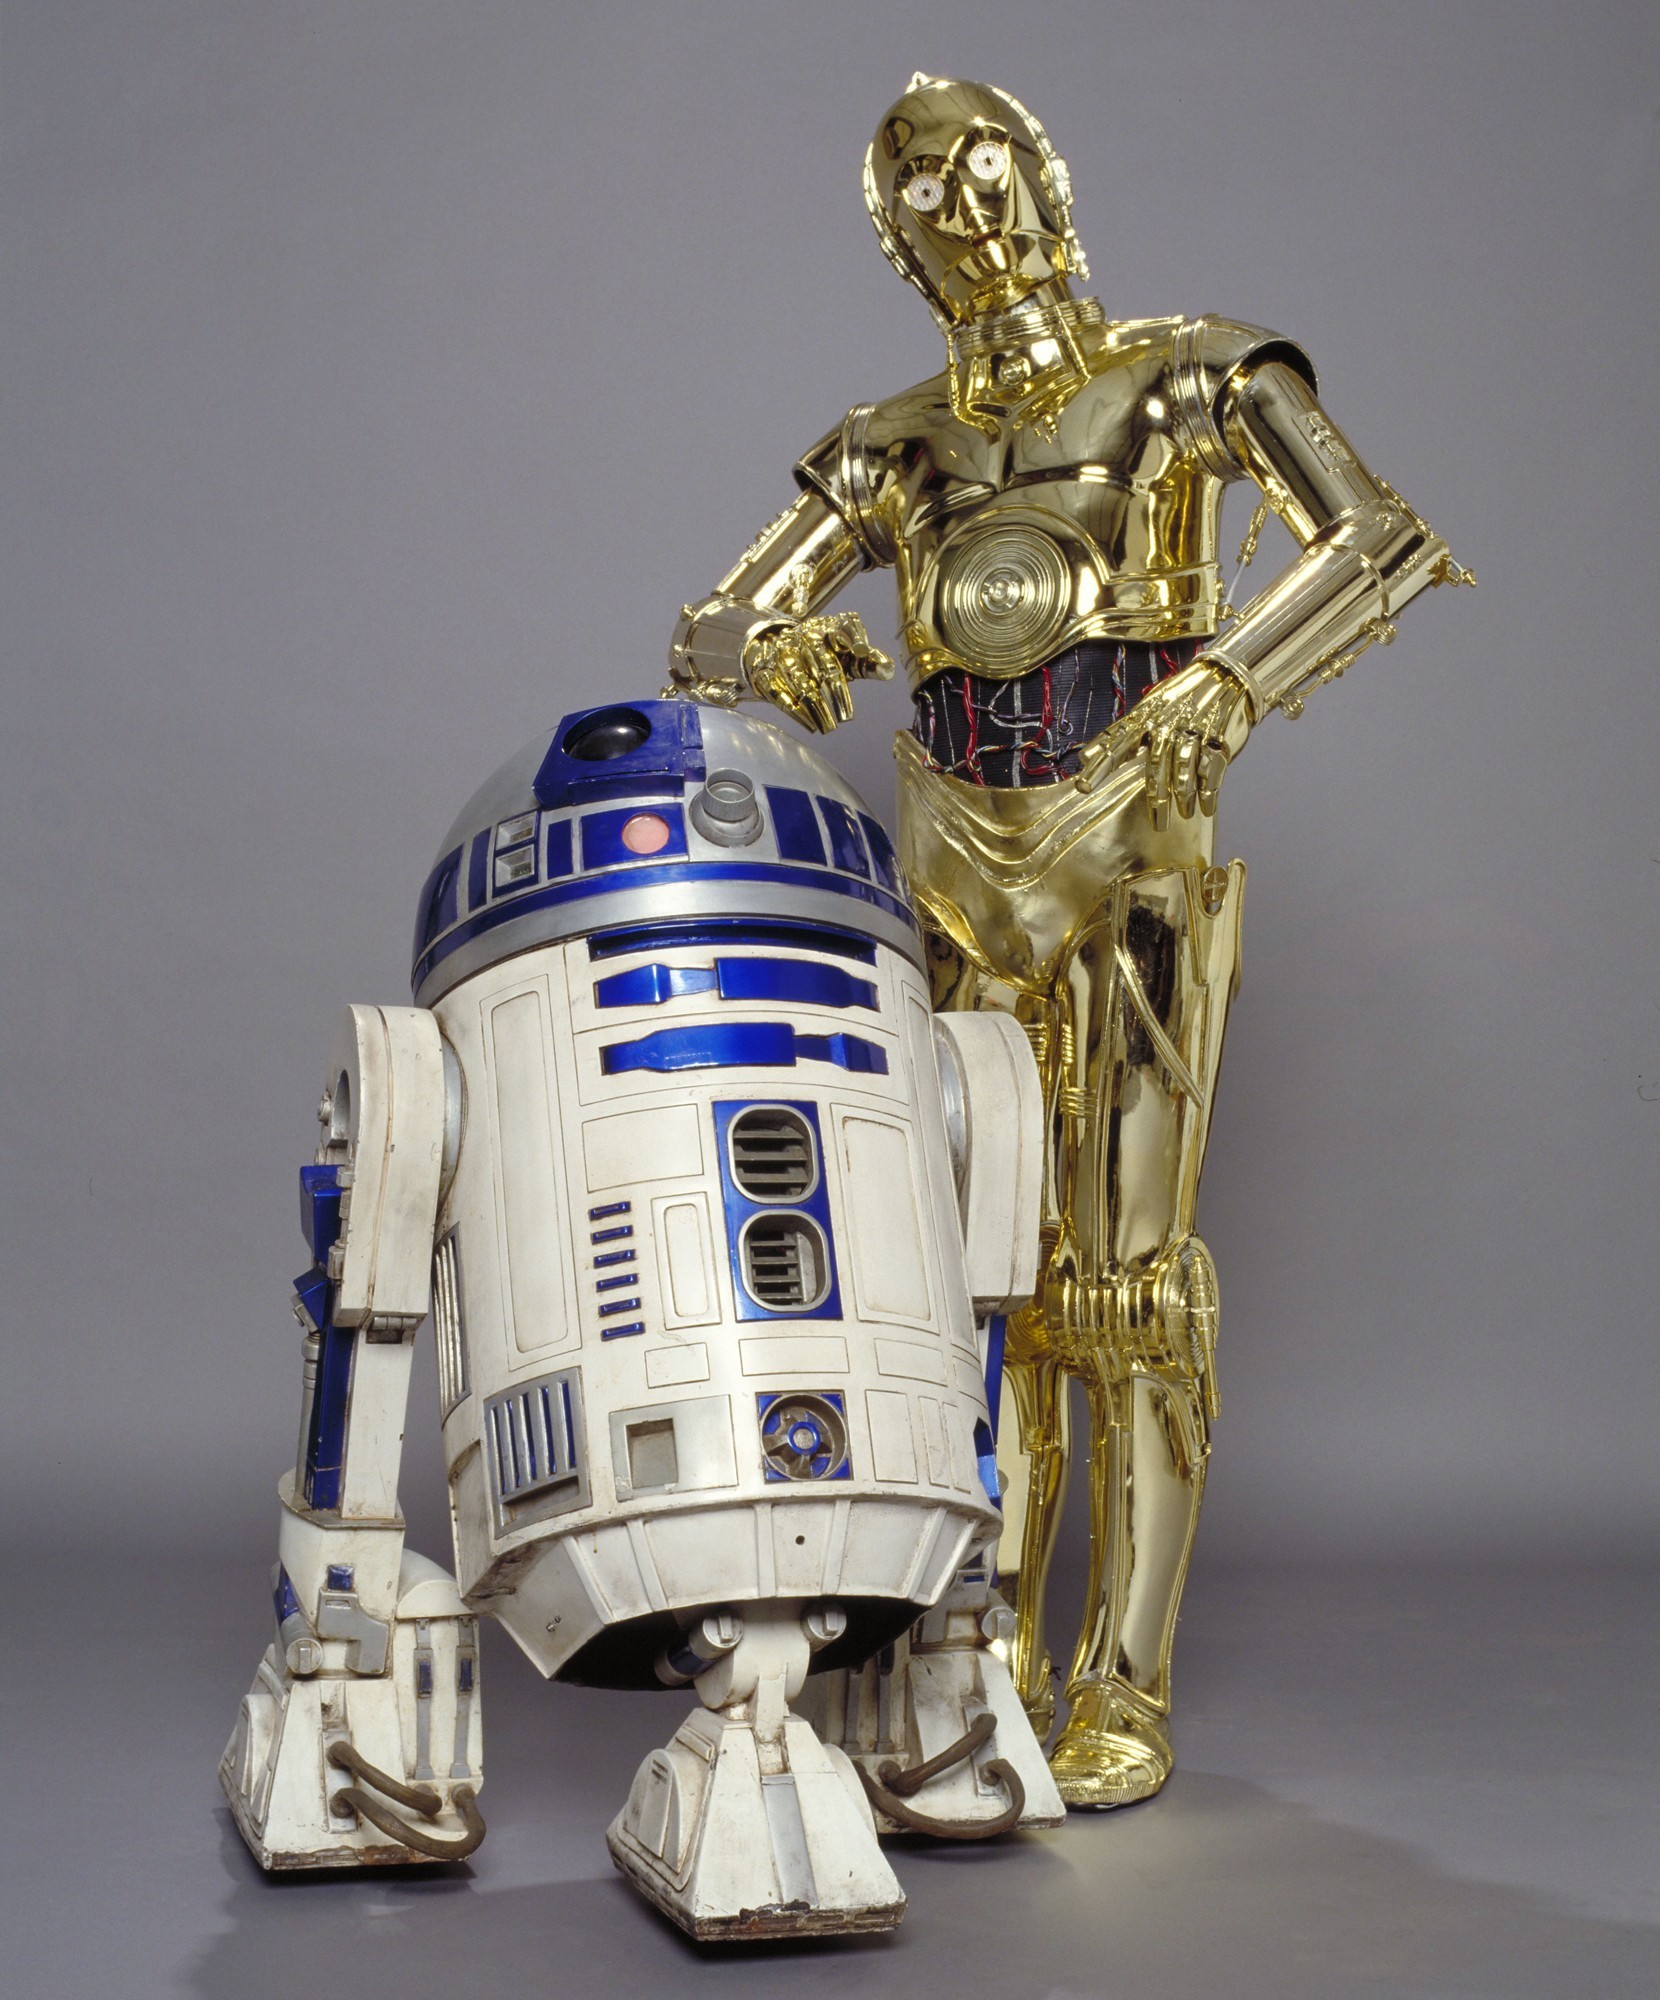
\includegraphics[height=3.00000cm]{imgs/starwars.jpg}
\caption{R2D2 et C3PO}
\end{figure}

\end{frame}

\section{Robotique Mobile}\label{robotique-mobile}

TODO: photo de r2d2

\subsection{B Robots mobiles
différentiels}\label{b-robots-mobiles-diffuxe9rentiels}

TODO

\begin{itemize}
\tightlist
\item
  Ken Hasselmann - ULB
\item
  Korantin Auguste - Google
\item
  Vincent Angladon - IRIT
\item
  Céleste Boursier-Mougenot
\end{itemize}

\begin{frame}{Fonctionnement}

Commençons par étudier les robots mobiles les plus simples: les robots
différentiels. Ces robots ont principalement deux roues parallèles dont
la vitesse est commandée indépendamment.

\begin{figure}
\centering
\includegraphics[height=2.00000cm]{tikz/differentiel.pdf}
\caption{Exemple de robot mobile différentiel}
\end{figure}

\pause

On peut donc contrôler indépendemment leurs vitesse linéaire et
angulaire.

\[
\begin{aligned}
v      &= \cfrac{\omega_r + \omega_l}{2} \cdot r \\
\omega &= \cfrac{\omega_r - \omega_l}{l} \cdot r
\end{aligned}
\]

\end{frame}

\begin{frame}{Application: \emph{offroad}}

Céleste Boursier-Mougenot est un artiste installationiste français. En
2013, il ous a demandé de travailler sur son œuvre \emph{offroad}.

\begin{figure}
\centering
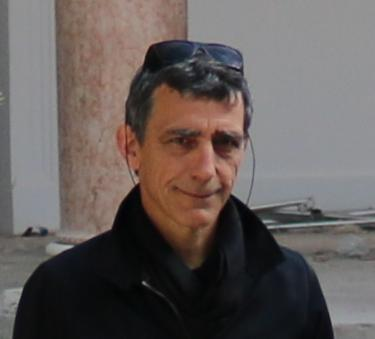
\includegraphics[height=2.00000cm]{imgs/celeste.jpg}
\caption{Céleste Boursier-Mougenot}
\end{figure}

\begin{itemize}
\tightlist
\item
  Trois pianos à queue doivent se mouvoir dans une salle
\item
  Au milieu du public
\item
  Ils peuvent se rentrer dedans et dans les murs
\item
  Leur mouvement doit être «esthétique» plutôt que «robotique»
\end{itemize}

\end{frame}

\subsection{C Robots mobiles à
tourelle}\label{c-robots-mobiles-uxe0-tourelle}

TODO

\begin{itemize}
\tightlist
\item
  BA Robotic Systems
\item
  Florent Lamiraux - LAAS-CNRS
\item
  Jean-Paul Laumond - LAAS-CNRS
\end{itemize}

\begin{frame}{Slide}

todo

\end{frame}

\subsection{D Robots mobiles
tri-tourelles}\label{d-robots-mobiles-tri-tourelles}

TODO

\begin{itemize}
\tightlist
\item
  BA Systèmes
\item
  Ubisense
\item
  Céleste Boursier-Mougenot
\item
  Michel Taïx - LAAS-CNRS
\item
  Jean-Paul Laumond - LAAS-CNRS
\end{itemize}

\begin{frame}{Slide}

todo

\end{frame}

\section{Robotique Humanoïde}\label{robotique-humanouxefde}

TODO: photo de c3po

\subsection{E Robots bipèdes}\label{e-robots-bipuxe8des}

TODO

\begin{itemize}
\tightlist
\item
  Gabriele Buondonno - Sapienza
\item
  Justin Carpentier - LAAS-CNRS
\item
  Nicolas Mansard - LAAS-CNRS
\item
  Alessandro De Luca - LAAS-CNRS
\item
  Jean-Paul Laumond - LAAS-CNRS
\end{itemize}

\begin{frame}{Slide}

todo

\end{frame}

\section{Conclusion}\label{conclusion}

\subsection{F Conclusion}\label{f-conclusion}

\begin{frame}{Slide}

todo

\end{frame}

\end{document}
% vim: set ft=tex:
